% ==========================================================
% ENTREGA 1 - O corpus do projeto
% Projeto Integrador III - Motor de Busca - Ciência de Dados
% Fatec Baixada Santista - Rubens Lara
% Equipe Shannon
% ==========================================================
%
% COMO COMPILAR
%   1. Na raiz: Rscript entregas/entrega-1/entrega-1-corpus.R
%      (gera os entrega-1-*.csv e entrega-1-numeros.txt nesta pasta)
%   2. Em entregas/entrega-1/: Rscript -e "knitr::knit2pdf('entrega-1-corpus.Rnw', bib_engine = 'bibtex')"
% ==========================================================

\documentclass[
  article,
  12pt,
  oneside,
  a4paper,
  english,
  brazil
]{abntex2}\usepackage[]{graphicx}\usepackage[]{xcolor}
% maxwidth is the original width if it is less than linewidth
% otherwise use linewidth (to make sure the graphics do not exceed the margin)
\makeatletter
\def\maxwidth{ %
  \ifdim\Gin@nat@width>\linewidth
    \linewidth
  \else
    \Gin@nat@width
  \fi
}
\makeatother

\definecolor{fgcolor}{rgb}{0.345, 0.345, 0.345}
\newcommand{\hlnum}[1]{\textcolor[rgb]{0.686,0.059,0.569}{#1}}%
\newcommand{\hlsng}[1]{\textcolor[rgb]{0.192,0.494,0.8}{#1}}%
\newcommand{\hlcom}[1]{\textcolor[rgb]{0.678,0.584,0.686}{\textit{#1}}}%
\newcommand{\hlopt}[1]{\textcolor[rgb]{0,0,0}{#1}}%
\newcommand{\hldef}[1]{\textcolor[rgb]{0.345,0.345,0.345}{#1}}%
\newcommand{\hlkwa}[1]{\textcolor[rgb]{0.161,0.373,0.58}{\textbf{#1}}}%
\newcommand{\hlkwb}[1]{\textcolor[rgb]{0.69,0.353,0.396}{#1}}%
\newcommand{\hlkwc}[1]{\textcolor[rgb]{0.333,0.667,0.333}{#1}}%
\newcommand{\hlkwd}[1]{\textcolor[rgb]{0.737,0.353,0.396}{\textbf{#1}}}%
\let\hlipl\hlkwb

\usepackage{framed}
\makeatletter
\newenvironment{kframe}{%
 \def\at@end@of@kframe{}%
 \ifinner\ifhmode%
  \def\at@end@of@kframe{\end{minipage}}%
  \begin{minipage}{\columnwidth}%
 \fi\fi%
 \def\FrameCommand##1{\hskip\@totalleftmargin \hskip-\fboxsep
 \colorbox{shadecolor}{##1}\hskip-\fboxsep
     % There is no \\@totalrightmargin, so:
     \hskip-\linewidth \hskip-\@totalleftmargin \hskip\columnwidth}%
 \MakeFramed {\advance\hsize-\width
   \@totalleftmargin\z@ \linewidth\hsize
   \@setminipage}}%
 {\par\unskip\endMakeFramed%
 \at@end@of@kframe}
\makeatother

\definecolor{shadecolor}{rgb}{.97, .97, .97}
\definecolor{messagecolor}{rgb}{0, 0, 0}
\definecolor{warningcolor}{rgb}{1, 0, 1}
\definecolor{errorcolor}{rgb}{1, 0, 0}
\newenvironment{knitrout}{}{} % an empty environment to be redefined in TeX

\usepackage{amsmath}
\usepackage{alltt}

\usepackage[T1]{fontenc}
\usepackage[utf8]{inputenc}
\usepackage{lmodern}
\usepackage{amsmath,amssymb}
\usepackage{icomma}
\usepackage{booktabs}
\usepackage[alf]{abntex2cite}

\hypersetup{hidelinks}
\setlength{\emergencystretch}{3em}

% ----------------------------------------------------------
% DADOS DA ENTREGA
% ----------------------------------------------------------
\titulo{O corpus do projeto: \textit{o Porto de Santos --- o lugar, a autoridade pública e o fundador}}
\tituloestrangeiro{}
\autor{Equipe Shannon}
\local{Santos-SP}
\data{\today}

\newcommand{\nomecurso}{Tecnologia em Ciência de Dados}
\newcommand{\nomedisciplina}{Projeto Integrador III --- Motor de Busca}
\newcommand{\nomeprofessor}{Prof.\ Dr.\ João Paulo Ferreira de Mello}
\newcommand{\repositorio}{projetointegrador3}
\newcommand{\integrantes}{%
  Adriane da Costa Santos (RA 0051352511040) \quad
  Danilo Prado de Lima Silva (RA 0051352521019) \\
  Victória Cabral Quintério (RA 0051352521033)%
}
\IfFileExists{upquote.sty}{\usepackage{upquote}}{}
\begin{document}





\selectlanguage{brazil}
\frenchspacing

\begin{center}
  \SingleSpacing
  {\Large \imprimirtitulo \par}
  \vspace{0.8em}
  {\large \imprimirautor \par}
  \vspace{0.3em}
  \imprimirlocal, \imprimirdata
\end{center}

\begin{center}
  \small
  \SingleSpacing
  Fatec Baixada Santista, Rubens Lara \quad|\quad \nomecurso{} \\
  \nomedisciplina{} \quad|\quad \nomeprofessor{} \\[0.3em]
  {\footnotesize \integrantes} \\[0.3em]
  Repositório: \texttt{\repositorio}
\end{center}

\textual

% ==========================================================================
\section{Introdução}
% ==========================================================================

O motor de busca do grupo é sobre o Porto de Santos, o mais movimentado da
América Latina e eixo econômico da Baixada Santista. Quem o usaria é um
estudante, jornalista ou analista que precisa achar \emph{a frase} que responde
a uma dúvida sobre o porto. O que se atende é a \emph{necessidade de
informação}, não a consulta literal \cite[cap.~1]{manning2008}; por isso as
perguntas vieram antes do corpus: \textbf{(1)} onde fica o porto; \textbf{(2)}
quem o administra hoje; \textbf{(3)} quem foi Francisco de Paula Ribeiro e
qual a sua ligação com o porto. Este texto apresenta a fonte, a coleta e a
evidência de que o corpus responde às três.

% ==========================================================================
\section{A fonte e o documento}
% ==========================================================================

O texto vem da Wikipédia em português, sob licença CC BY-SA, de três páginas:
\textit{Porto de Santos} \cite{wikiporto}, \textit{Autoridade Portuária de
Santos} \cite{wikiaps} e \textit{Francisco de Paula Ribeiro}
\cite{wikiribeiro}, salvas em agosto de 2026: o \textbf{lugar}, a
\textbf{autoridade pública} e o \textbf{fundador}, uma para cada pergunta.
São $N = \text{122}$ documentos.

Um documento é \textbf{uma frase pontuada}, \texttt{dN.k} (página \texttt{N},
frase \texttt{k}): a menor unidade que responde sozinha a uma pergunta. O
artigo inteiro diria só ``está no artigo do porto'', e o parágrafo --- padrão do
curso --- daria \text{18} documentos, abaixo da faixa e
misturando assuntos. A frase \texttt{d1.1}, ``Porto de Santos é um porto estuarino, localizado nos municípios de Santos, Guarujá e\ldots'', responde
sozinha à pergunta~1.

A motivação foi o conhecimento prévio: o grupo já estuda o porto em Teoria do
Aprendizado Estatístico, com dados da ANTAQ --- a alternativa descartada, por
serem tabelas numéricas, não prosa.

% ==========================================================================
\section{Como o corpus foi obtido}
% ==========================================================================

O corpo de cada artigo, sem infobox nem referências, foi salvo em UTF-8 em
\texttt{estrutura/corpus/} (19/08/2026). O script \texttt{01a-ler-frases.R}
quebra o texto por \texttt{.}, \texttt{!} e \texttt{?} (e \texttt{;} acima de
45 palavras), descarta fragmentos de menos de 3 palavras e numera as frases em
\texttt{frases-canonicas.csv}, com os mesmos IDs da Aula 01 à 05.

\textbf{O que deu errado.} (i) O artigo inteiro como documento dava só 3
documentos. (ii) Cortes fixos de 7 a 10 palavras partiam frases, e os juízes
não julgavam sem contexto; passou-se à pontuação. (iii) Abreviações e decimais
(\texttt{S.A.}, \texttt{1,5}) quebravam frases e passaram a ser protegidas.
(iv) Fragmentos de 1 ou 2 palavras foram descartados.

% ==========================================================================
\section{Defesa do corpus}
% ==========================================================================

\begin{table}[htb]
  \centering
  \caption{Diagnóstico do corpus (tokenização bruta da Aula 01)}
  \label{tab:diag}
  \small
  \begin{tabular}{@{}p{0.30\textwidth}p{0.62\textwidth}@{}}
    \toprule
    \textbf{Verificação} & \textbf{Resultado} \\
    \midrule
    Tamanho                & \text{122} documentos (frases) de \text{3} páginas \\
    Tokens por documento   & \text{6} a \text{76} (média 28,6, mediana 25,5) \\
    Vocabulário bruto      & 1.281 termos em 3.493 tokens (\text{873} radicais após a Aula 03) \\
    Por página             & frases (parágrafos): \textit{Porto de Santos} 88 (12); \textit{Autoridade Portu\'aria} 29 (5); \textit{Paula Ribeiro} 5 (1) \\
    Página que domina      & \textit{Porto de Santos}: \text{88} de \text{122} (72\%) \\
    Documentos suspeitos   & \text{0} com menos de \text{5} tokens; \text{1} com mais de \text{60} (\texttt{d1.66}) \\
    Sujeira                & \text{119} com acento, \text{122} com pontuação, \text{59} com dígitos (de \text{122}) \\
    \bottomrule
  \end{tabular}
  \fonte{Elaborada pelos autores (\texttt{entrega-1-corpus.R}).}
\end{table}

\textbf{Tamanho.} São \text{122} documentos (Tabela~\ref{tab:diag}),
acima da meta de 20 a 60, por causa da unidade: em parágrafos seriam
\text{18}. A frase fica, pois já foi indexada e julgada.
\textbf{Domínio.} O porto tem 72\% do corpus e o
fundador só \text{5} frases: é a cara do tema,
mas a pergunta 3 depende de poucas frases; a correção é acrescentar páginas.
\textbf{Não prosa.} A única frase acima de \text{60} tokens,
\texttt{d1.66}, é uma lista de terminais que perdeu as quebras de
linha; por ser longa, é o 1.º lugar do TF-IDF na pergunta 2, e o BM25, que
normaliza pelo tamanho, a tira do top-5 \cite{robertson2009}.
\textbf{Sujeira.} Acentos, pontuação grudada e \text{59} frases
com dígitos: o esperado, tratado na Aula 03. Pela Figura~\ref{fig:tam}, a
maioria das frases tem de 15 a 40 tokens.

\begin{figure}[htb]
  \centering
  \caption{Tokens por documento}
  \label{fig:tam}
\begin{knitrout}
\definecolor{shadecolor}{rgb}{0.969, 0.969, 0.969}\color{fgcolor}

{\centering 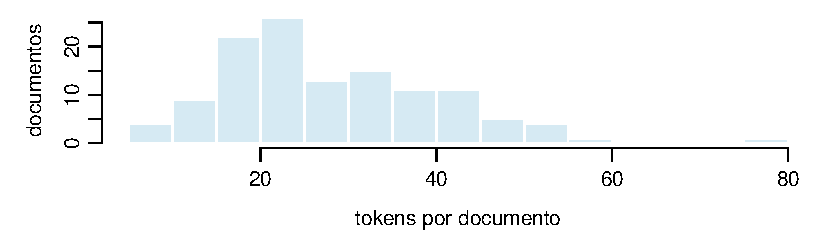
\includegraphics[width=0.5\linewidth]{figure/fig-tam-1} 

}


\end{knitrout}
  \fonte{Elaborada pelos autores.}
\end{figure}

\textbf{Os termos mais frequentes} são \texttt{de}, \texttt{a}, \texttt{e}, \texttt{o}, \texttt{da}, \texttt{do}, \texttt{porto}, \texttt{em}, \texttt{que}, \texttt{com}: só
\texttt{porto} fala do tema; o resto é o que as \textit{stopwords} removem.

\textbf{Veredito.} Na Tabela~\ref{tab:busca}, as perguntas 1 e 3 têm a
resposta (\texttt{d1.1}, \texttt{d3.1}, grau 2) em 1.º lugar em todos os
métodos ranqueados. Na pergunta 2 o nDCG é zero por defeito do gabarito, não
do corpus: \texttt{d2.4}, ``Desde então, a APS administra a infraestrutura pública do Porto de\ldots'', responde e fica em 3.º no
cosseno e no BM25, mas recebeu grau~0 dos dois juízes, em 1 e 4 segundos. O AND
não devolve nada; o OR devolve metade do corpus.

\begin{table}[htb]
  \centering
  \caption{As três perguntas no corpus: documentos devolvidos e nDCG@5}
  \label{tab:busca}
  \small
  \begin{tabular}{@{}lrrcrrr@{}}
    \toprule
    Pergunta & AND & OR & 1.º lugar & TF-IDF & Cosseno & BM25 \\
    \midrule
    1. Onde fica o porto     & \text{0} & \text{60} & \texttt{d1.1} & 0,64 & 0,72 & 0,74 \\
    2. Quem administra       & \text{0} & \text{69} & \texttt{d1.36} & 0,00 & 0,00 & 0,00 \\
    3. Quem foi o fundador   & \text{0} & \text{52} & \texttt{d3.1} & 0,76 & 0,76 & 0,76 \\
    \midrule
    Tempo médio (ms)         & 1,2 & 1,4 & & 1,2 & 3,0 & 1,4 \\
    \bottomrule
  \end{tabular}
  \fonte{Elaborada pelos autores. 1.º lugar do BM25; nDCG@5 com os graus 0/1/2 de \texttt{05-qrels.csv} \cite{jarvelin2002}; tempo médio de 200 execuções por consulta.}
\end{table}

O corpus contém a resposta às três perguntas e é \textbf{provisório}: antes
de congelar o gabarito, o grupo vai rejulgar a pergunta 2, quebrar
\texttt{d1.66} em itens e acrescentar uma página sobre a Companhia
Docas de Santos.

\postextual
{\SingleSpacing\footnotesize
\bibliography{referencias}}

\end{document}
